%%%%%%%%%%%%%%%%%%%%%%%%%%%%%%%%%%%%%%%%%%%%%%%%%%%%%%%%%%%%%%
% --> INTRODUCCIÓN
%%%%%%%%%%%%%%%%%%%%%%%%%%%%%%%%%%%%%%%%%%%%%%%%%%%%%%%%%%%%%%
\section{Introducción}

El concepto de medir la complejidad computacional de un problema, analizando la cantidad de recursos computacionales necesarios para solucionar un problema, como lo son:

\begin{itemize}
    \item Espacio
    \item Tiempo
\end{itemize}

El rendimiento o complejidad, está ligado únicamente al algoritmo. En ningún momento con la velocidad del computador o con las facilidades de eficiencia que presenta un lenguaje de programación, ni con el estilo hábil del programador.

Para calcular este rendimiento se tiene en cuenta dos pasos principales:

\begin{enumerate}
    \item Caracterizar las operaciones básicas del algoritmo: operaciones básicas son las que constituyen el trabajo realizado para resolver el problema. Si el algoritmo ejecuta una estructura repetitiva (ciclo), la básico en el proceso no es la actualización del índice para la satisfacción de la condición.
    \item Debe considerarse sobre quien va a recaer la operación. Se considera entonces los datos, de los datos debe considerarse el tamaño y la configuración. 
\end{enumerate}

Por lo tanto en este laboratorio a se habla de la teoría de la complejidad computacional, que básicamente  estudia los recursos requeridos para resolver un problema como son el tiempo y el espacio; por su parte la teoría de la computabilidad se interesa en expresar los problemas como algoritmos sin tener en cuenta la información sobre los recursos necesarios para ello.


%%%%%%%%%%%%%%%%%%%%%%%%%%%%%%%%%%%%%%%%%%%%%%%%%%%%%%%%%%%%%%
% --> OBJETIVOS
%%%%%%%%%%%%%%%%%%%%%%%%%%%%%%%%%%%%%%%%%%%%%%%%%%%%%%%%%%%%%%
\subsection{Objetivos}



%%%%%%%%%%%%%%%%%%%%%%%%%%%%%%%%%%%%%%%%%%%%%%%%%%%%%%%%%%%%%%
% --> OBJETIVO GENERAL
%%%%%%%%%%%%%%%%%%%%%%%%%%%%%%%%%%%%%%%%%%%%%%%%%%%%%%%%%%%%%%
\subsubsection{Objetivo General}
\begin{itemize}
\item Estudiar conceptos básicos de complejidad computacional y análisis de
algoritmos.
\end{itemize}

%%%%%%%%%%%%%%%%%%%%%%%%%%%%%%%%%%%%%%%%%%%%%%%%%%%%%%%%%%%%%%
% --> OBJETIVOS ESPECÍFICOS
%%%%%%%%%%%%%%%%%%%%%%%%%%%%%%%%%%%%%%%%%%%%%%%%%%%%%%%%%%%%%%
\subsubsection{Objetivos Específicos}
\begin{itemize}
\item Comprender y ejemplificar el concepto de problemas NP.
\item Comprender y ejemplificar el concepto de problemas NP-duros.
\item Comprender y ejemplificar el concepto de problemas NP-completos.
\item Realizar el análisis de un problema para obtener la función de tiempo de ejecución y la complejidad del programa. 
\end{itemize}

%%%%%%%%%%%%%%%%%%%%%%%%%%%%%%%%%%%%%%%%%%%%%%%%%%%%%%%%%%%%%%
% --> ENUNCIADO
%%%%%%%%%%%%%%%%%%%%%%%%%%%%%%%%%%%%%%%%%%%%%%%%%%%%%%%%%%%%%%
%\newpage

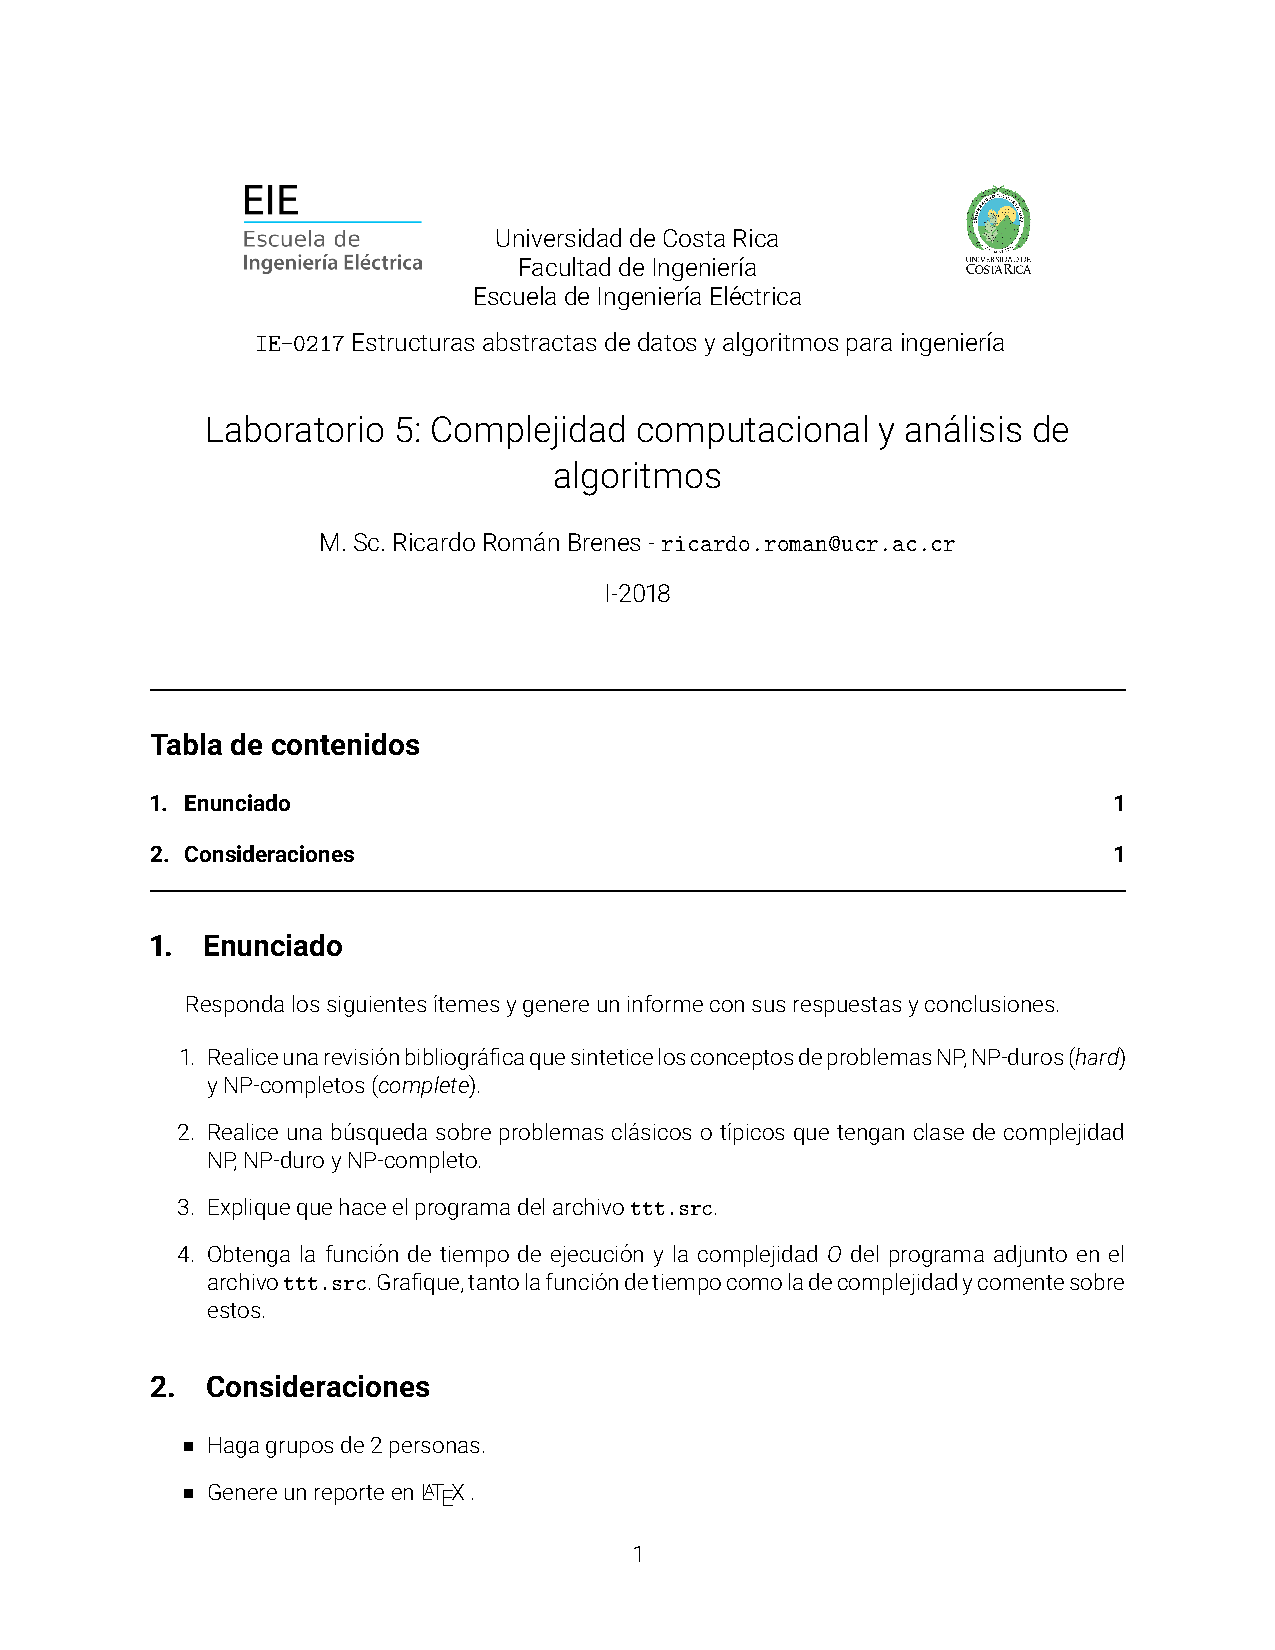
\includepdf[pages=1,pagecommand=\section{Enunciado}, scale=0.8]{enunciados/enun5} 
\includepdf[pages=2,pagecommand={},scale=0.8]{enunciados/enun5}

%%%%%%%%%%%%%%%%%%%%%%%%%%%%%%%%%%%%%%%%%%%%%%%%%%%%%%%%%%%%%%
% --> SOLUCIÓN
%%%%%%%%%%%%%%%%%%%%%%%%%%%%%%%%%%%%%%%%%%%%%%%%%%%%%%%%%%%%%%
\section{Solución}

\subsection{Clases de complejidad computacional}

Como se mencionó anteriormente, la complejidad computacional es una rama de la teoría de la computación, y se encarga de medir la dificultad para computar una función en términos de los recursos requeridos, principalmente tiempo y espacio \cite{R3}. Esta teoría plantea una clasificación en \emph{clases}, según la dificultad inherente de los problemas.

Por lo general, un método que se utilice para resolver un problema de decisión se denomina \textit{algoritmo}. Un algoritmo \textbf{de tiempo polinomial} es aquel cuyo tiempo de ejecución crece en función del tamaño de su entrada como una función polinomial \cite{R4}.

%%%%%%%%%%%%%%%%%%%%%%%%%%%%%%%%%%%%%%%%%%%%%%%%%%
%-----------------------------------
\subsection{Problemas NP}
%-----------------------------------

En complejidad computacional se pueden presentar problemas no deterministas, estos son problemas que se resuelven en tiempo polinomial no determinista y pertenecen a la clase de problemas denominada NP. Estos problemas son resueltos por una hipotética máquina de Turing no determinista que es capaz de resolver entre dos posibles salidas o soluciones\cite{R8}, es decir, una máquina que tiene la capacidad de elegir cuál camino es más eficiente o conveniente para el problema. Es importante comentar que la clase de complejidad NP se dice que es una generalización de la clase P, por lo que todos los problemas P son problemas NP, pero no al contrario\cite{R6}.

\subsubsection{Ejemplos de problemas de clase NP}

Los problemas NP abarcan los problemas NP-Hard y NP-Complete, por eligieron problemas representativos para la clase.
\begin{itemize}
    \item \textbf{Problema de la coloración de grafos:} Este problema consiste en colorear los vértices de un grafo de tal manera que ningún vértice adyacente comparta el mismo color. Además se busca la menor cantidad posible de colores que se pueden utilizar para colorear un grafo dado\cite{R9}.
    
    \item \textbf{Problema de la mochila: } Este problema consiste en llenar una mochila con objetos que tienen dos características: peso y valor. El problema se da en que la mochila solo soporta una cantidad limitada de peso, por lo que se busca cargarla con los objetos que maximicen el valor, pero que no sobrepasen el peso máximo soportado por la mochila \cite{R9}. Este tipo de problemas se clasifican en una categoría denominada optimización combinatoria.
\end{itemize}
%%%%%%%%%%%%%%%%%%%%%%%%%%%%%%%%%%%%%%%%%%%%%%%%%%

%-----------------------------------
\subsection{Problemas NP-hard}
%-----------------------------------
%En la clase NP-Hard son todos aquellos problemas en NP que puede ser polinometicamante reducidos 
%La clase de problemas NP-Hard, por lo general requieren de una solución exponencial e inclusive peor. 
La clase de los problemas NP-hard como la clases de los problemas tales que si fuesen polinómicos se verificaría P = NP. Nuevamente se utiliza la técnica de la reducibilidad para demostrar que un problema es NP-hard, pues si un problema NP-completo es reducible a otro problema, entonces el segundo es NP-hard. Aplicando esta técnica se encuentran problemas de optimización que son NP-duros, y más en general que ciertos problemas de búsqueda son NP-duros.

Básicamente los problemas NP-hard no tienen algoritmos polinomiales por lo que un algoritmo que los resuelva en forma exacta puede tardar un tiempo prohibitivo. 

%-----------------------------------
\subsubsection{Ejemplos de problemas de clase NP-hard}
%-----------------------------------
\begin{itemize}
    \item \textbf{Closest string}:\\
    Este problemas trata de encontrar el centro geométrico de un conjunto de cadenas de entrada. Más formalmente, dado $n$ longitud-$m$ strings $s_1$ , $s_2$ , ..., $s_n$ , el problema de cadena más cercano busca una nueva longitud $m$ cadena s tal que $d ( s , s_i ) \leq k$ para todo $i$ , donde $d$ denota la distancia de Hamming , y donde $k$ es lo más pequeño posible.
    \item \textbf{Travelling salesman problem}:\\
    Dada una lista de ciudades y las distancias entre cada par de ciudades, ¿cuál es la ruta más corta posible que visita cada ciudad y regresa a la ciudad de origen? Es un problema NP-hard en la optimización combinatoria, importante en la investigación de operaciones y la informática teórica.
\end{itemize}

%%%%%%%%%%%%%%%%%%%%%%%%%%%%%%%%%%%%%%%%%%%%%%%%%%
%-----------------------------------
\subsection{Problemas NP-Complete}
%-----------------------------------

Existe una clase de problemas NP, de la que se dice que no se conoce su estado. Esto quiere decir que no se ha descubierto ningún algoritmo de tiempo polinomial que resuelva un problema de este tipo, pero tampoco se ha comprobado que no pueda existir alguno \cite{R5}. Se afirma, además, que si \textbf{algún} problema de tipo NP-C se puede resolver en tiempo polinomial, entonces \textbf{cualquier} problema de tipo NP es solucionable con un algoritmo de tiempo polinomial.

%-----------------------------------
\subsubsection{Ejemplos de problemas de clase NP-complete}
%-----------------------------------
\begin{itemize}
    \item \textbf{Problema de satisfacibilidad booleana} \cite{R7}: \\
    Los elementos de una fórmula booleana son variables booleanas, $x_1,x_2,...\in{0,1}$; operadores $\wedge$ (conjunción o AND), $\vee$ (disyunción o OR) y $\neg$ (negación o NOT); y paréntesis. Se le denomina \textbf{cláusula} a una disyunción de uno o más variables.\\
    Se dice que una fórmula booleana está en la \textbf{forma normal conjuntiva}, si es una conjunción de dos o más cláusulas. Por ejemplo, $\phi = (x_1\vee x_2 \vee \neg x_3)\wedge(x_2\vee \neg x_3 \vee x_4) \wedge (\neg x_1 \vee x_2 \vee x_5)$
\end{itemize}

\subsection{Análisis del programa en el archivo \texttt{theCode.src}}

El código proporcionado corresponde a un juego de "gato". El programa cuenta con una estructura de datos \texttt{TicTacToe()} que inicializa una matriz $nxn$. También se dispone de una función \texttt{move()} que se encarga de marcar la posición en donde se encuentra el jugador, y a su vez comprueba si ya hay tres casillas consecutivas llenas por el mismo jugador, es decir, comprueba si el juego termina porque el jugador ganó.

\texttt{TicTacToe} se inicializa con una matriz cuadrada vacía, de un tamaño \texttt{n} que se le pasa como parámetro. 

\begin{minted}[linenos,autogobble,bgcolor=bg,breaklines,fontsize=\footnotesize ]{c++}
public class TicTacToe {
 
    int[][] matrix;
 
    /** Initialize your data structure here. */
    public TicTacToe(int n) {
        matrix = new int[n][n];
    }
\end{minted} 

El método \texttt{move} recibe como parámetros una posición de la matriz mediante las variables \texttt{row} (fila) y \texttt{col} (columna), y el jugador cuyo turno se va a ejecutar. La movida consiste simplemente en colocar el valor de \texttt{player} en la posición indicada de la matriz (línea 2).
Luego se realizan chequeos para determinar si después de la movida algún jugador ganó. Se revisa si hay tres valores iguales de \texttt{player} consecutivos en dirección horizontal (línea 5), vertical (línea 16) y las diagonales (líneas 27 y 38), y el resultado (verdadero o falso) se le asigna a la variable \texttt{win}.

La variable \texttt{win} determina el valor que retorna la función, si hubo algún ganador retorna el valor del jugador ganador (\texttt{player}), en caso contrario retorna 0.

\begin{minted}[linenos,autogobble,bgcolor=bg,breaklines,fontsize=\footnotesize ]{c++}
    int move(int row, int col, int player) {
        matrix[row][col]=player;
 
        //check row
        boolean win=true;
        for(int i=0; i<matrix.length; i++){
            if(matrix[row][i]!=player){
                win=false;
                break;
            }
        }
 
        if(win) return player;
 
        //check column
        win=true;
        for(int i=0; i<matrix.length; i++){
            if(matrix[i][col]!=player){
                win=false;
                break;
            }
        }
 
        if(win) return player;
 
        //check back diagonal
        win=true;
        for(int i=0; i<matrix.length; i++){
            if(matrix[i][i]!=player){
                win=false;
                break;
            }
        }
 
        if(win) return player;
 
        //check forward diagonal
        win=true;
        for(int i=0; i<matrix.length; i++){
            if(matrix[i][matrix.length-i-1]!=player){
                win=false;
                break;
            }
        }
 
        if(win) return player;
 
        return 0;
    }

}
\end{minted}


En el programa principal se inicializan los elementos que van a conformar el juego: \texttt{player} indica el jugador de turno, \texttt{end} ayudará a detectar el fin del juego, \texttt{n=3} el tamaño de la matriz sobra la que se creará el juego, \texttt{r} y \texttt{c} la posición en fila y columna. Luego se crea una instancia de la clase \texttt{TicTacToe} de tamaño \texttt{n}. En un ciclo while, se alterna el turno de jugadores (línea 12) y se busca una posición aleatoria dentro de la matriz. Luego se realiza la movida mediante el método \texttt{move}, cuyo valor de retorno se asigna a la variable \texttt{result}. La variable \texttt{end} indica el fin del ciclo cuando se haya obtenido un ganador.


\begin{minted}[linenos,autogobble,bgcolor=bg,breaklines,fontsize=\footnotesize ]{c++}
public class TicTacToe {    
    int main()
    {
        int player = -1;
        boolean end = false;
        int n = 3;
        int r, c, result;
        
        TicTacToe ttt = new TicTacToe(n);
        while(!end)
        {
            player *= -1
            r =  randomInt(0, 3);
            c =  randomInt(0, 3);
            
            result = move(player, r, c);
            if(result != 0)
            {
                print("player " + result + " won.");
                end = true;
            }
        }
        return 0;
    }
\end{minted}

%%%%%%%%%%%%%%%%%%%%%%%%%%%%%%%%%%%%%%%%%%%%%%%%%%%%%%%%%%%%%%
% --> RESULTADOS
%%%%%%%%%%%%%%%%%%%%%%%%%%%%%%%%%%%%%%%%%%%%%%%%%%%%%%%%%%%%%%
\section{Resultados}

Para calcular las funciones de tiempo $T(n)$ y la de complejidad $O(n)$ se calcularon los pasos necesarios para que se resuelva un problema de tamaño $n$. En el código inferior se observan los valores tomados para cada línea del código de la clase \texttt{TicTacToe()} y de la función \texttt{move()}. En donde el valor más importante se presenta en el ciclo \texttt{for} dentro de la función mencionada anteriormente, este ciclo a porta un valor $n$ correspondiente a las veces que se va a ejecutar. Como el programa realiza esa comparación para comprobar las filas, columnas y las diagonales, se presenta 4 veces $n$, por lo tanto para esta sección de código se tendría una función de tiempo $T_1(n)=4n+22$. 

\begin{minted}[linenos,autogobble,bgcolor=bg,breaklines,fontsize=\footnotesize ]{c++}
int[][] matrix;->declaracion(1)
    public TicTacToe(int n) {
        matrix = new int[n][n];->declaracion(1)	
    }
    int move(int row, int col, int player) {				
        matrix[row][col]=player; ->declaracion(1)
        boolean win=true; ->asignacion (1)
        for(int i=0; i<matrix.length; i++){->(asignacion (1), comparacion (1), incrremento (1) ) x n veces
            if(matrix[row][i]!=player){ ->comparacion (1)
                win=false; ->asignacion(1)
                break; ->(1)
            }
        }
        if(win) return player; ->(1)
    .
    .
    .
        return 0; ->(1)
    }		
\end{minted}

Para la sección del \texttt{main()} se realizó el mismo procedimiento, en donde destaca el aporte de $n$ por parte del ciclo \texttt{while}; así como el hecho de que se presente la función \texttt{move()} dentro del \texttt{while}, por esto, se tiene una función de tiempo $T_2(n)=8+n(6+T_1(n))$. Entonces realizando la sustitución se tiene la función de tiempo total: 

\begin{equation*}
    T(n) = 4n^2+28n+8
\end{equation*}

Además, para calcular la función de complejidad se desprecian los coeficientes y se mantiene únicamente el valor más grande de $n$, por lo que se tiene:

\begin{equation*}
    O(T(n)) = O(n^2)
\end{equation*}

\begin{minted}[linenos,autogobble,bgcolor=bg,breaklines,fontsize=\footnotesize ]{c++}
int main()
    {
        int player = -1; ->asignacion(1)
        boolean end = false;->asignacion(1)
        int n = 3;->asignacion(1)
        int r, c, result;->inicializacion(3)
        TicTacToe ttt = new TicTacToe(n);->asignacion(1)
        while(!end)	->ejecucion(n){
            player *= -1;->asignacion(1)
            r =  randomInt(0, 3);->asignacion(1)
            c =  randomInt(0, 3);->asignacion(1)
            result = move(player, r, c);->(4n+22)
            if(result != 0)->(1){
                print("player " + result + " won.");->(1)
                end = true;->asignacion(1)
            }
        }
        return 0;->(1)
    }
}
\end{minted}

Una vez obtenidas ambas funciones se procede a graficarlas como se observa en la Figura \ref{fig:OnTn}.

\begin{figure}[H]
\centering
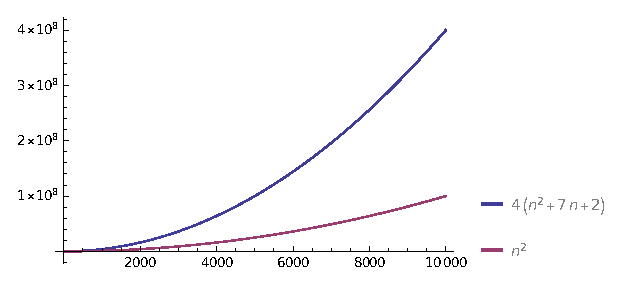
\includegraphics[width=\textwidth]{imgs/Labo5/plot.eps}
\caption{Gráficas de la función de tiempo $T(n)$ y la función de complejidad $O(n)$.}
\label{fig:OnTn}
\end{figure}

%%%%%%%%%%%%%%%%%%%%%%%%%%%%%%%%%%%%%%%%%%%%%%%%%%%%%%%%%%%%%%
% --> CONCLUSIONES
%%%%%%%%%%%%%%%%%%%%%%%%%%%%%%%%%%%%%%%%%%%%%%%%%%%%%%%%%%%%%%
\section{Conclusiones}


Como conclusiones se tiene que:

\begin{itemize}
%\item Existen varias clases de complejidad computacional, que sirven para describir la dificultad de ejecutar un algoritmo en términos de los recursos utilizados. 
\item Se encontró que dentro de las clases de complejidad temporal, NP describe problemas de decisión que se pueden resolver en tiempo polinomial por una Máquina de Turing no-determinista.
\item Se analizó un programa en pseudocódigo para determinar su función de tiempo de ejecución y su complejidad O.
\item Se determinó que el programa estudiado tiene complejidad cuadrática ($O(n^2)$) y se graficó su función de tiempo de ejecución y su complejidad.
\end{itemize}


%%%%%%%%%%%%%%%%%%%%%%%%%%%%%%%%%%%%%%%%%%%%%%%%%%%%%%%%%%%%%%
% --> BIBLIOGRAFIA
%%%%%%%%%%%%%%%%%%%%%%%%%%%%%%%%%%%%%%%%%%%%%%%%%%%%%%%%%%%%%%
\begin{thebibliography}{IEEE}

\bibitem{R3} Immerman, N. \textbf{\textit{Computational complexity classes}}. Encyclopedia of Mathematics, 2011. Visto el 7 de mayo en \url{https://www.encyclopediaofmath.org/index.php/Computational_complexity_classes}

\bibitem{R4} Kaliski B.  \textbf{\textit{Polynomial Time}}. Encyclopedia of Cryptography and Security. Springer, Boston, MA, 2005.

\bibitem{R5} Cormen, T., Leiserson, C., Rivest, R. y Stein, C. \textbf{\textit{Introduction to Algorithms}}. Tercera Ed. Massachusetts Institute of Technology, 2009.

\bibitem{R6} Papadimitriu, C.H., \textbf{\textit{Computational Complexity}}. Encyclopedia of Computer Science, Cuarta Ed, páginas 260-265. John Wiley and Sons Ltd. Chichester, UK, 2003.


\bibitem{R7} Witmer, D. \textbf{\textit{Lecture 36: NP-Completeness}}. Abril, 2017. Visto el 7 de mayo del 2018 es: \url{http://www.cs.cmu.edu/afs/cs/academic/class/15750-s17/ScribeNotes/lecture36.pdf}


\bibitem{R8} Papadimitriu, C.H., Lewis, H. \textbf{\textit{Elements of Theory of Computation}}. Segunda Ed, páginas 292-294. Prentice Hall, New Jersey, 1998.

\bibitem{R9} Karp, R. \textbf{\textit{Reducibility Among Combinatorial Problems}}. Primera Ed, Universidad de California, 1972.

\end{thebibliography}

